% !Mode:: "TeX:UTF-8"
\documentclass{article}
% !Mode:: "TeX:UTF-8"
\usepackage[english]{babel}
\usepackage[UTF8]{ctex}
\usepackage{amsmath, amsthm, amssymb}

% Figure
\usepackage{graphicx}
\usepackage{float} %% H can fix the location
\usepackage{caption}
\usepackage[format=hang,singlelinecheck=0,font={sf,small},labelfont=bf]{subfig}
\usepackage[noabbrev]{cleveref}
\captionsetup[subfigure]{subrefformat=simple,labelformat=simple,listofformat=subsimple}
\renewcommand\thesubfigure{(\alph{subfigure})}

\usepackage{epstopdf} %% convert eps to pdf
\DeclareGraphicsExtensions{.eps,.mps,.pdf,.jpg,.png} %% bmp, gif not supported
\DeclareGraphicsRule{*}{eps}{*}{}
\graphicspath{{img/}{figure/}{../figure/}} %% fig directorys

%% \usepackage{pstricks} %% a set of macros that allow the inclusion of PostScript drawings directly inside TeX or LaTeX code
%% \usepackage{wrapfig} %% Wrapping text around figures

% Table
\usepackage{booktabs} %% allow the use of \toprule, \midrule, and \bottomrule
\usepackage{tabularx}
\usepackage{multirow}
\usepackage{colortbl}
\usepackage{longtable}
\usepackage{supertabular}

\usepackage[colorinlistoftodos]{todonotes}

% Geometry
\usepackage[paper=a4paper, top=1.5cm, bottom=1.5cm, left=1cm, right=1cm]{geometry}
%% \usepackage[paper=a4paper, top=2.54cm, bottom=2.54cm, left=3.18cm, right=3.18cm]{geometry} %% ms word
%% \usepackage[top=0.1cm, bottom=0.1cm, left=0.1cm, right=0.1cm, paperwidth=9cm, paperheight=11.7cm]{geometry} %% kindle

% Code
%% \usepackage{alltt} %% \textbf can be used in alltt, but not in verbatim

\usepackage{listings}
\lstset{
    backgroundcolor=\color{white},
    columns=flexible,
    breakatwhitespace=false,
    breaklines=true,
    captionpos=tt,
    frame=single, %% Frame: show a box around, possible values are: none|leftline|topline|bottomline|lines|single|shadowbox
    numbers=left, %% possible values are: left, right, none
    numbersep=5pt,
    showspaces=false,
    showstringspaces=false,
    showtabs=false,
    stepnumber=1, %% interval of lines to display the line number
    rulecolor=\color{black},
    tabsize=2,
    texcl=true,
    title=\lstname,
    escapeinside={\%*}{*)},
    extendedchars=false,
    mathescape=true,
    xleftmargin=3em,
    xrightmargin=3em,
    numberstyle=\color{gray},
    keywordstyle=\color{blue},
    commentstyle=\color{green},
    stringstyle=\color{red},
}

% Reference
%% \bibliographystyle{plain} % reference style

% Color
\usepackage[colorlinks, linkcolor=blue, anchorcolor=red, citecolor=green, CJKbookmarks=true]{hyperref}
\usepackage{color}
\def\red#1{\textcolor[rgb]{1.00,0.00,0.00}{#1}}
\newcommand\warning[1]{\red{#1}}

% Other
%% \usepackage{fixltx2e} %% for use of \textsubscript
%% \usepackage{dirtree}  %% directory structure, like the result of command tree in bash shell

   %导入需要用到的package
% !Mode:: "TeX:UTF-8"
%+++++++++++++++++++++++++++++++++++article+++++++++++++++++++++++++++++++++
%customize the numbering of equation, to make it like section-subsection-equation style, for example,1-2-3
\makeatletter\@addtoreset{equation}{subsection}\makeatother
\renewcommand\theequation{%
\thepart\arabic{section}%
-\thepart\arabic{subsection}%
-\thepart\arabic{equation}%
}
%theorem
\newtheorem{definition}{D\'efintion} %% 整篇文章的全局编号
\newtheorem*{thmwn}{Thm} %% without numbers
\newtheorem{theorem}{Th\'eor\`eme}[section] %% 从属于section编号
\newtheorem{corollary}{Corollary}[theorem] %% 从属于theorem编号
\newtheorem{lemma}{Lemma}
\newtheorem{proposition}{Proposition}[section]
\newtheorem{example}{Example}
\newtheorem*{attention}{Attention}
\newtheorem*{note}{Note}
\newtheorem*{remark}{Remark}
\newtheorem{question}{Question}[section]
\newtheorem{problem}{Problem}
\newtheorem{fact}{Fact}

   %导入需要用到的package
\begin{document}
\title{Introduction to algorithm \\Eric's Notes}
\author{Eric}
\maketitle
\newpage
\tableofcontents
\newpage

\section{课程简介及算法分析}
\subsection{Insertion sort}
Pseudocode
\begin{verbatim}
INSERTION-SORT(A)
1 for j ← 2 to length[A]  #1是第一个元素
2 	do key ← A[j] //将将要插入的数据保存下来
3 	//Insert A[j] into the sorted sequence A[1 _ j - 1].
4	 i ← j - 1
5	 while i > 0 and A[i] > key
6		 do A[i + 1] ← A[i]
7		 i ← i - 1
8	 A[i + 1] ← key
\end{verbatim}
\begin{figure}[htbp]
  \centering
  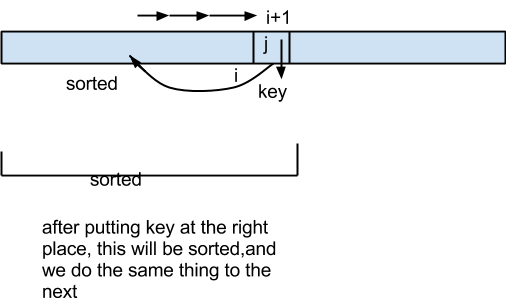
\includegraphics[scale = 0.7]{sort_insertion}\\
  \caption{Insertion sort}\label{fig.sort.insertion}
\end{figure}

ex:
\begin{verbatim}
8 2 4 9 3 6
2 8 4 9 3 6 // 2 goes before 8
2 4 8 9 3 6 // 4 goes before 8
2 4 8 9 3 6 // 9 stays there
2 3 4 8 9 6 // 3 goes before 4
2 3 4 6 8 9 // 6 goes before 8
\end{verbatim}

\begin{figure}[htbp]
  \centering
  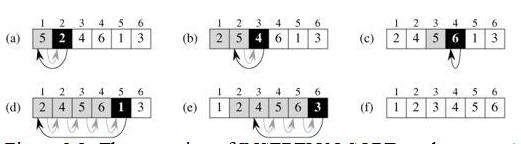
\includegraphics[scale = 0.7]{sort_insertion_example}\\
  \caption{Insertion sort}\label{fig.sort.insertion.example}
\end{figure}

python code
\begin{verbatim}
def insertionSort(L):
	#in place algorithem, 升序
	for j in range(1,len(L)):
		#将将要排序的数据保存下来, 开始对第j 个元素进行排序
		key=L[j]
		i=j-1
		#找到存放key的位置
		while i >= 0 and L[i]>key:
			L[i+1]=L[i] ## 将大数往后移动
			i=i-1
		##循环结束,说明L[i] <= key,所以key应该放在i+1处
		L[i+1]=key
	return L
\end{verbatim}

running time\\
1 already sorted: 最理想情况\\
2 reverse sorted: 最差情况

we want upper bounds 上界

kinds of analysis\\
worst-case $T(n)=max$ time of any input of size n\\
average-case $T(n)=expected time$期望时间\\
(need assumption of statistical  distribution of inputs)\\
best-case (bogus假象)

BIG IDEA: \textbf{asymptotic analysis渐进分析}\\
not the the exact running time of an algorithm\\
the order of growth of the running time

the insertion sort analysis\\
worst-case: input reverse sorted
$$T(n)=\sum_{j=2}^{j=n} \theta(j)=\theta(n^2) \eqnote{算术级数arithmetic series}$$

\subsection{Merge sort}
算法\\
T(n) merge sort A[1...n]\\
$\theta(1)$	1 if n=1, done\\
$2 \times \theta(n/2)$	2 Recursively sort A[1...upper(n/2)] and A[upper(n/2)+1...n]    向上取整\\
$\theta(n)$	3 merge 2 sorted  list

Merge\\
Where is the smallest element of any two lists that are already sorted?\\
It is in one of two places, the head of the first list or the head of the second list

\textbf{Key subroutine Merge}
\begin{verbatim}
2 7 13 20
1 9 11 12
\end{verbatim}
在两个list head中,1最小,所以1是n个元素中最小的,排在最终的list的第一个位置,现在总list和两个子list成为:
\begin{verbatim}
1
2 7 13 20
9 11 12
\end{verbatim}
然后在比较两个子list 中head位置那个更小,把它放在总list的第二个位置
\begin{verbatim}
1 2
7 13 20
9 11 12
\end{verbatim}
一直这么继续下去,
这里的每一步都是固定数目的操作,和每一步中的数组的尺寸无关,每一步总,我们只关注两个head,并挑出最小的,再把数组指针推进一位,所以我知道当前的标头在哪里.
所以,对于总数为n的输入,时间是$\theta(n)$的
所以把两个list遍历和排序的时间是$\theta(n)$,有时我们称之为线性时间

merge sort的例子
\begin{figure}[htbp]
  \centering
  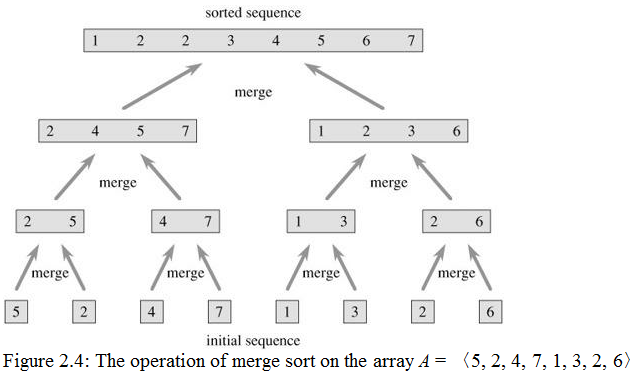
\includegraphics[scale = 0.7]{sort_merge_example}\\
  \caption{Merge sort example}\label{fig.sort.merge.example}
\end{figure}

时间复杂度
$$
T(n) =
\left\{
  \begin{array}{ll}
	\theta(1) \si n=1 \\
	2 \times T(n/2) + \theta(n) \si n>1
  \end{array}
\right.
$$

\subsection{Recursion tree}
一直做下去,得到,每一行的和都为$cn$,数的深度为$\lg n$,树的level是$\lg n+1$,最后一层的叶节点有$n$个,每一个都是$\theta(1)$

\begin{figure}[htbp]
  \centering
  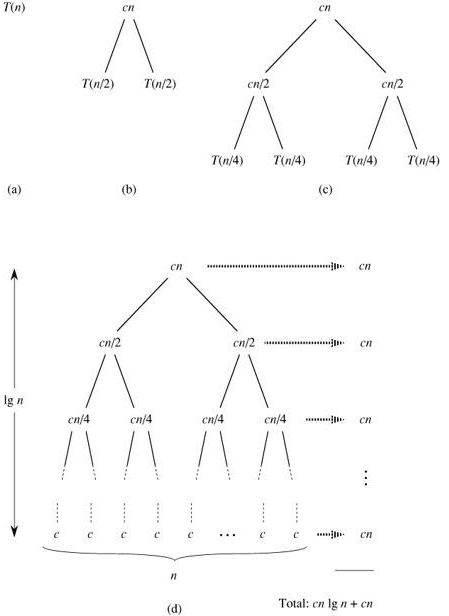
\includegraphics[scale = 0.7]{recursion_tree}\\
  \caption{Recursion tree example}\label{fig.compute.recursion_tree}
\end{figure}

为了便于计算,我们在这里设$\theta(1)=c$;
先把每一层的加起来,得到都是$cn$,然后再把所有层加起来,得到
$$T(n)=(\lg n +1)cn=\Theta(n\lg n )$$
So merge sort beats insertion sort.
$$ \theta(n\lg n )<\theta(n^2) $$

\section{渐进符号,递归及解法}
\begin{definition}
\begin{figure}[htbp]
  \centering
  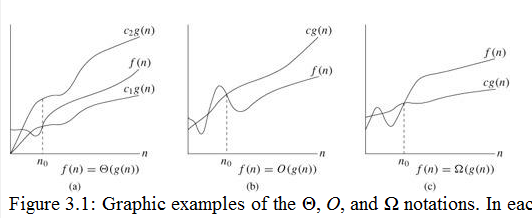
\includegraphics[scale = 0.7]{notation_asymptotical}\\
  \caption{Asymptotical notation}\label{fig.notation.asymptotical}
\end{figure}
\textbf{BIG O:上界 <=}\\
$O(g(n)) = \{f(n): $there exist positive constants $c$ and $n_0$ such that $0 \leq f(n) \leq cg(n)$ for all $n \geq n_0\}$\\
We say that $g(n)$ is an asymptotically upper bound for $f(n)$

\textbf{BIG $\Omega$下界 >=}\\
$\Omega(g(n)) = \{f(n): $there exist positive constants $c$ and $n_0$ such that $0\leq cg(n)\leq f(n)$ for all $n geq n_0\}$\\
We say that $g(n)$ is an asymptotically lower bound for $f(n)$.

\textbf{BIG $\Theta$ =}\\
$\Theta(g(n)) = \{f(n) : $there exist positive constants $c_1, c_2$, and $n_0$ such that $0\leq c\lg n\leq f(n)\leq c_2g(n)$ for all $n geq n_0\}$\\
$$\Theta(g(n))=O(g(n)) \cap \Omega(g(n)) $$\\
We say that $g(n)$ is an asymptotically tight bound for $f(n)$.

The definition of $\Theta(g(n))$ requires that every member $f(n) in \Theta(g(n))$ be asymptotically nonnegative, that is, that $f(n)$ be nonnegative whenever $n$ is sufficiently large.
\end{definition}

Ex:
$2n^2 + \Theta(n) = \Theta(n^2)$
for any function $f(n) in \Theta(n)$, there is some function $g(n) in \Theta(n^2)$ such that $2n^2 + f(n) = g(n)$ for all $n$. In other words, the right-hand side of an equation provides a coarser level of detail than the left-hand side.

o-notation
to denote an upper bound that is not asymptotically tight.\\
$o(g(n)) = \{f(n) : $for any positive constant $c > 0$, there exists a constant $n_0 > 0$ such that $0 \leq f(n) < cg(n)$ for all $n geq n_0\}$\\
For example, $2n = o(n^2)$, but $2n^2 \neq o(n^2)$

o-notation表示的是一种相差比较大的\\
in the o-notation, the function $f(n)$ becomes insignificant relative to $g(n)$ as $n$ approaches infinity; that is,
$$\lim_{n \to \infty} \frac{f(n)}{g(n)} = 0 $$

ω-notation
By analogy, ω-notation is to ?-notation as o-notation is to O-notation.
$$ \lim_{n \to \infty} \frac{f(n)}{g(n)} = \infty $$

\textbf{Comparison of functions}\\
与数的比较类比
\begin{itemize}
	\item $f(n) = O(g(n))	\approx	a \leq b$
	\item $f(n) = \Omega(g(n))	\approx a \geq b$
	\item $f(n) = \Theta(g(n))	\approx	a = b$
	\item $f(n) = o(g(n))	\approx	a \ll b$
	\item $f(n) = \omega(g(n))	\approx	a \gg b$
\end{itemize}

\subsection{Standard notations and common functions}
函数的单调性\\
monotonically increasing单调增\\
monotonically decreasing\\
strictly increasing严格递增\\
strictly decreasing

Floors and ceilings
$$
x -1 < \lfloor x \rfloor \leq x \leq \lceil x \rceil < x + 1
$$

For any integer $n, \lceil n/2 \rceil + \lfloor n/2 \rfloor = n$

And for any real number $n \geq 0$ and integer $a,b >0$
\begin{enumerate}
	\item $\lceil \lceil n/a \rceil /b \rceil = \lceil n/(ab) \rceil$
	\item $\lfloor \lfloor n/a \rfloor /b \rfloor = \lfloor n/(ab) \rfloor$
	\item $\lceil a/b \rceil \leq (a+(b-1))b$
	\item $\lfloor a/b \rfloor \geq (a-(b-1))/b$
	\item $a \mod n = a - \lfloor a/n \rfloor n$
\end{enumerate}

$\lim_{n \to \infty} \dfrac{n^b}{a^n} = 0$
from which we can conclude that
$n^b = o(a^n)$.
Thus, any exponential function with a base strictly greater than $1$ grows faster than any polynomial function.

$$
\lim_{n \to \infty} \frac{\lg ^b n}{(2^a)^{\lg n}} = \lim_{n \to \infty}\frac{\lg ^b n}{n^a} = 0
$$
$\lg^bn = o(n^a)$,
for any constant $a > 0$. Thus, any positive polynomial function grows faster than any polylogarithmic function.
$$
n! = \sqrt{2\pi n} (\frac{n}{e})^n (1 + \Theta(\frac{1}{n}))
$$
Functional iteration\\
We use the notation $f(i)(n)$ to denote the function $f(n)$ iteratively applied $i$ times to an initial value of $n$. Formally, let $f(n)$ be a function over the reals. For nonnegative integers $i$, we recursively define
$$
f^{(i)}(n) =
\left\{
  \begin{array}{ll}
		  n & \si i = 0\\
		  f(f^{(i-1)}(n)) & \si i >0
  \end{array}
\right.
$$
For example, if $f(n) = 2n$, then $f^{(i)}(n) = 2^in$.

\subsection{Substitution method}
Substitution method for solving recurrences entails two steps:\\
Guess the form of the solution.\\
Use mathematical induction(数学归纳法) to find the constants and show that the solution works.

Ex:
$T(n) = 2T(\lfloor n/2 \rfloor) + n$\\
猜测$T(n) = O(n \lg n)$,然后归纳法证明

$T(n) = 2T(n/2 + 17) + n$
与上一式相差$17$,但是当$n$很大时,$17$可以忽略掉,所以仍然猜测$T(n) = O(n \lg n)$,然后尝试用归纳法证明,发现是正确的

\subsubsection{Subtleties}
$T(n) = T(n/2) + T(n/2) + 1$.\\
我们猜测$T(n) \leq cn$\\
$T(n) \leq c n/2 + c n/2 + 1 =cn + 1$ ,wrong,但是只差了一个常数\\
we're only off by the constant 1, a lower-order term,加上一个lower-order term,猜测$T(n) \leq cn - b$\\
$T(n) \leq (c n/2 - b) + (c n/2- b) + 1 = cn - 2b + 1 \leq cn - b$\\
imply $b \geq 1$,所以当$b \geq 1$时,$T(n) \leq cn - b$

\subsubsection{Changing variables}
$T(n) = 2T(\lfloor \sqrt{n} \rfloor) +\lg n$\\
Renaming $m = \lg n$ yields  $T(2^m) = 2T(2^m/2) + m$.\\
We can now rename $S(m) = T(2^m)$ to produce the new recurrence
$S(m) = 2S(m/2) + m$,\\
这个见过,$S(m) = O(m \lg m)$.\\
Changing back from $S(m)$ to $T(n)$, we obtain
$$
T(n) = T(2^m) = S(m) = O(m \lg m) = O(\lg n \lg \lg n).
$$

\subsection{Recursion-tree method}
In a recursion tree, each node represents the cost of a single subproblem somewhere in the set of recursive function invocations.

We sum the costs within each level of the tree to obtain a set of per-level costs, and then we sum all the per-level costs to
determine the total cost of all levels of the recursion.

Recursion trees are particularly useful when the recurrence describes the running time of a divide-and-conquer algorithm.

A recursion tree is best used to generate a good guess,
which is then verified by the substitution method. So we can often tolerate a small amount of "sloppiness", since you will be verifying your guess later on.

Ex:
$T(n) = 3T(n/4) + \Theta(n^2)$\\
We create a recursion tree for the recurrence: $T(n) = 3T(n/4) + cn^2$,如图\ref{fig.compute.recursion_tree2}所示
\begin{figure}[htbp]
  \centering
  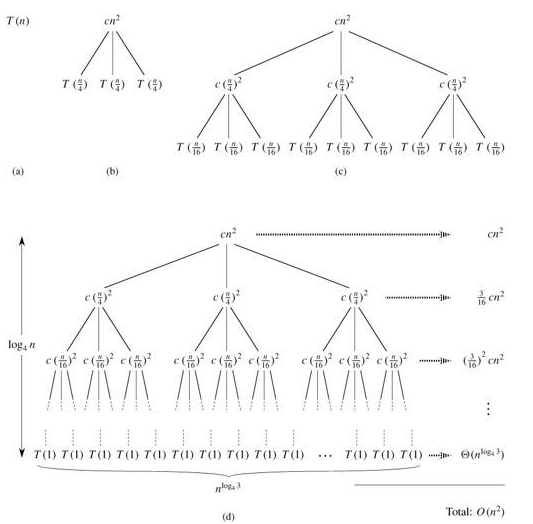
\includegraphics[scale = 0.7]{recursion_tree2}\\
  \caption{Recursion tree example}\label{fig.compute.recursion_tree2}
\end{figure}

Assume that n is an exact power of 4 (another example of tolerable sloppiness)\\
Its height is $\log_4 n$ (it has $\log_4 n + 1$ levels ($0, 1, 2,..., \log_4 n$))\\
The subproblem size for a node at depth i is $n/4^i$.\\
Each level has three times more nodes than the level above, and so the number of nodes at depth $i$ is $3i$.

深度为 $i = 0, 1, 2,..., \log_4 n - 1$,的nodes加起来 is $3^i c(n/4^i)^2 = (3/16)^icn^2$.\\
最后一层,at depth $\log_4n$, has $3^{\log_4 n} = n^{\log_4 3}$ nodes, each contributing cost $T(1)$, for a total cost of $n^{\log_4 3}T(1)$ , which is $\Theta(n^{\log_4 3})$.\\
把所有层的加起来,得到整个树的时间
\begin{equation}
\begin{split}
		T(n) & = cn^2 + \frac{3}{16} cn^2 + (\frac{3}{16})^2 cn^2 + \dots + (\frac{3}{16})^{\log_4 n - 1}cn^2 + \Theta(n^{\log_4 3}) \\
				   & = \sum_{i=0}^{\log_4 n - 1}(\frac{3}{16})^i cn^2 + \Theta(n^{\log_4 3}) \\
				   & = \frac{(3/16)^{\log_4 n} - 1}{(3/16)-1} cn^2 + \Theta(n^{\log_4 3})
\end{split}
\end{equation}
保留高阶项,得到$T(n)=O(n^2)$,
然后再用归纳法证明,发现是正确的

\subsection{Master method}
Theorem:Let $a \geq 1$ and $b > 1$ be constants, let $f(n)$ be a asymptotically positive function, and let $T(n)$ be defined on the nonnegative integers by the recurrence
$$T(n) = aT(n/b) + f(n)$$
Where we interpret $n/b$ to mean either $\lceil n/b \rceil$ or $\lfloor n/b \rfloor$. Then $T(n)$ can be bounded asymptotically as follows.
\begin{enumerate}
	\item If $f(n) = O(n^{\log_b a - \epsilon})$ for some constant $\epsilon > 0$, then $T(n) = \Theta(n^{\log_b a})$
	\item If $f(n) = n^{\log_{b} a}$, then $T(n) = \Theta(n^{\log_b a} \lg n)$
	\item If $f(n) = n^{\log_{b} a + \epsilon}$ for some constant $\epsilon > 0$, and if $a f(n/b) \leq cf(n)$ for some constant $c < 1$ and all sufficiently large $n$, then $T(n) = \Theta(f(n))$.
\end{enumerate}

总结规律如下:
Compare the function $f(n)$ with the function  $n^{\log_b a}$\\
if $f(n)$ is polynomial smaller, case $1$\\
if $f(n)$ is polynomial lager, case $3$

It is important to realize that \textbf{these three cases do not cover all the possibilities for} $f(n)$.
There is a gap between cases $1$ and $2$ when $f(n)$ is smaller than $n^{\log_b a}$ but not polynomially smaller.
Similarly, there is a gap between cases $2$ and $3$ when $f(n)$ is larger than $n^{\log_b a}$ but not polynomially larger.
If the function $f(n)$ falls into one of these gaps, or if the regularity condition in case $3$ fails to hold,
the master method cannot be used to solve the recurrence.

Ex: $T(n) = 3T(n/4) + n \lg  n$,\\
we have $a = 3, b = 4, f (n) = n \lg  n$,\\
$f(n)/(n^{\log_b a})=n\lg n/(n^{\log_4 3})=n^{1 - \log_4 3} \times \lg n$\\
so $f(n)$ is polynomial lager, case $3$, $T(n) = \Theta(n\lg  n)$.

\subsubsection{Proof of master method}
树的深度是$\log_b n$
图示证明见\ref{fig.compute.recursion_tree.proof}
\begin{figure}[htbp]
  \centering
  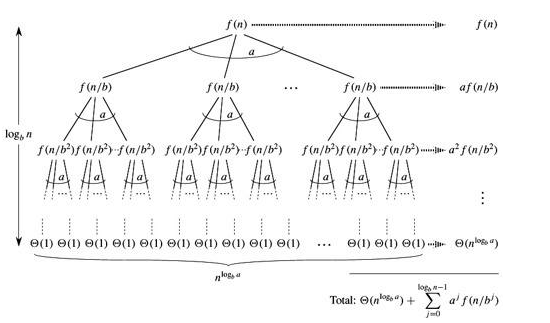
\includegraphics[scale = 0.7]{recursion_tree_proof}\\
  \caption{Recursion tree proof}\label{fig.compute.recursion_tree.proof}
\end{figure}
不太严格的证明,但是有助于理解\par
case 3:前面是呈几何级数递减的,所以前面所有层的和 is dominated by the first member $f(n)$\\
最后一层的和为$a^(\log_b n) \times  \Theta(1)=n^(\log_b a) \Theta(1)= \Theta(n^(\log_b a))$\\
$T(n)=\Theta(f(n))$\\
所以比较$f(n) and (n^(\log_b a))$也就是比较最后一层与前面所有层的

case 1:前面是呈几何级数递增的,因为$f(n)$ is polynomial smaller than $n^(\log_b a)$,所以整个求和中,$n^(\log_b a)$占据主导\\
$T(n)=\Theta(n^(\log_b a))$

case 2: 由于最顶层和最底层的差不多,在中间的,从最顶层呢过到最底层变化又不大,所以基本上都一个量级的,所以总和是:\\
$T(n)=(\log_b n+1)f(n)=(\log_b n+1) \times n^(\log_b a)=\Theta(f(n) \times \lg n)$

\section{分治法 divide and conquer}
The divide-and-conquer design paradigm
\begin{enumerate}
	\item Divide the problem (instance) into subproblems.
	\item Conquer the subproblems by solving them recursively.
	\item Combine subproblem solutions
\end{enumerate}

\subsection{Merge sort}
\begin{enumerate}
	\item Divide:Trivial.
	\item Conquer:Recursively sort 2 subarrays.
	\item Combine:Linear-time merge.
\end{enumerate}
$$
T(n)=2 \times T(n/2) +\Theta(n)=\Theta(n\lg n)
$$

\subsection{Binary serach}
find x in \textbf{sorted array}
\begin{enumerate}
	\item divide, compare x with middle
	\item conquer : recurse in one subarray
	\item combine: trivial
\end{enumerate}
$$
T(n)=\Theta(1)+1 \times T(n/2) = \Theta(\lg n)	\eqnote{master method}
$$

Algorithm $BinarySearch(L; x; first; last)$\\
Input: Array $L[first ; last]$ and value $x$.\\
Output: $1$ if $x \in L$, or $i$, $0<=  i < n$ if $L[i] = x$

pseudo code\\
if $first > last$ then return $-1$\\
else \{\\
$middle \leftarrow (first+last)/2$\\
if $L[middle]=x$ then return $middle$\\
else if $L[middle]<x$ then return $BinarySearch(L; x; middle+1; last)$\\
else return $BinarySearch(L; x; first; middle - 1)$\\
\}

\subsection{Powering a number}
given number $x$, integer $n \geq 0$, compute $x^n$\\
general method:$x \times x \times x \times x \times \cdots \times x =x^n$,  $T(n)=\Theta(n)$

Divide and conquer:
$$
x^n =
\left\{
  \begin{array}{ll}
		  x^{n/2} \times x^{n/2}  \eqnote{if n even}\\
	x^{(n-1)/2} \times x^{(n-1)/2} \times x \eqnote{if n odd}
  \end{array}
\right.
$$
$T(n)=1 \times T(n/2) +\Theta(1)=\Theta(\lg n)$\\
$T(n/2)$表示算出平方根的时间,$\Theta(1)$表示将这个算出来的平方根平方的时间

\subsection{Fibonacci numbers}
$F_0=0,F_1=1,F_2=1,F_3=3.....$\\
通式:$F_n=F_{n-1} + F_{n-2}$\\
General method: $T(n)=\Omega(\phi^n)$ with $\phi=(1+\sqrt{5})/2$
golden ratio\\
exponential time

\textbf{bottom-up}\\
Compute $F_0,F_1,F_2,....$ in order\\
当我们要计算$F_n$的时候,我们已经计算出了$F_{n-1}$ and $F_{n-2}$,直接将这两个相加,就得到$F_n$, 将两个已知数相加所需要的时间为常数\\
所以只需要依次计算各个项就可以了\\
$T(n)=n \times \Theta(1)=\Theta(n)$

\textbf{Naive recursive squaring}\\
根据Fibonacci通项公式,直接计算,and round to the nearest integer\\
但是浮点数的计算误差比较大

\textbf{Recursive squaring}
\begin{theorem}
$$
\left(
  \begin{array}{cc}
		  F_{n+1} & F_n \\
		  F_n & F_{n-1}
  \end{array}
\right)
=
\left(
  \begin{array}{cc}
		  1 & 1 \\
		  1 & 0
  \end{array}
\right)^n
$$
\end{theorem}
prove the matrix equation by induction on n
$T(n)=T(n/2)+\Theta(1)$
$T(n)=\Theta(\lg n)$

\subsection{Matrix multiplication}
input $A=a_{ij}, B=b_{ij}$\\
output $C=A \times B$\\
Standard algorithm
\begin{verbatim}
for i ←1 to n
	do for j←1 to n
			do cij←0
			for k←1 to n
				do cij←cij+ aik \times bkj
\end{verbatim}
直接计算,三层嵌套循环,时间复杂度是$\Theta(n^3)$

divide and conquer algo:\\
直接分治法
$n×n$ matrix = $2×2$ matrix of $(n/2)×(n/2)$ submatrices:

$$
\mathbf{A} =
\begin{bmatrix}
\mathbf{A}_{1,1} & \mathbf{A}_{1,2} \\
\mathbf{A}_{2,1} & \mathbf{A}_{2,2}
\end{bmatrix}
\mbox { , }
\mathbf{B} =
\begin{bmatrix}
\mathbf{B}_{1,1} & \mathbf{B}_{1,2} \\
\mathbf{B}_{2,1} & \mathbf{B}_{2,2}
\end{bmatrix}
\mbox { , }
\mathbf{C} =
\begin{bmatrix}
\mathbf{C}_{1,1} & \mathbf{C}_{1,2} \\
\mathbf{C}_{2,1} & \mathbf{C}_{2,2}
\end{bmatrix}
$$
with
$$
\mathbf{A}_{i,j}, \mathbf{B}_{i,j}, \mathbf{C}_{i,j} \in R^{2^{n-1} \times 2^{n-1}}
$$
then
$$
\begin{aligned}
\mathbf{C}_{1,1} = \mathbf{A}_{1,1} \mathbf{B}_{1,1} + \mathbf{A}_{1,2} \mathbf{B}_{2,1} \\
\mathbf{C}_{1,2} = \mathbf{A}_{1,1} \mathbf{B}_{1,2} + \mathbf{A}_{1,2} \mathbf{B}_{2,2} \\
\mathbf{C}_{2,1} = \mathbf{A}_{2,1} \mathbf{B}_{1,1} + \mathbf{A}_{2,2} \mathbf{B}_{2,1} \\
\mathbf{C}_{2,2} = \mathbf{A}_{2,1} \mathbf{B}_{1,2} + \mathbf{A}_{2,2} \mathbf{B}_{2,2}
\end{aligned}
$$
With this construction we have not reduced the number of multiplications.
We still need $8$ multiplications to calculate the $C_{i,j}$ matrices, the same number of multiplications we need when using standard matrix multiplication.

Now comes the important part. We define new matrices
$$
\begin{aligned}
& \mathbf{M}_{1} := (\mathbf{A}_{1,1} + \mathbf{A}_{2,2}) (\mathbf{B}_{1,1} + \mathbf{B}_{2,2})\\
& \mathbf{M}_{2} := (\mathbf{A}_{2,1} + \mathbf{A}_{2,2}) \mathbf{B}_{1,1}\\
& \mathbf{M}_{3} := \mathbf{A}_{1,1} (\mathbf{B}_{1,2} - \mathbf{B}_{2,2})\\
& \mathbf{M}_{4} := \mathbf{A}_{2,2} (\mathbf{B}_{2,1} - \mathbf{B}_{1,1})\\
& \mathbf{M}_{5} := (\mathbf{A}_{1,1} + \mathbf{A}_{1,2}) \mathbf{B}_{2,2}\\
& \mathbf{M}_{6} := (\mathbf{A}_{2,1} - \mathbf{A}_{1,1}) (\mathbf{B}_{1,1} + \mathbf{B}_{1,2})\\
& \mathbf{M}_{7} := (\mathbf{A}_{1,2} - \mathbf{A}_{2,2}) (\mathbf{B}_{2,1} + \mathbf{B}_{2,2})
\end{aligned}
$$
only using $7$ multiplications (one for each $M_k$) instead of $8$. We may now express the $C_{i,j}$ in terms of $M_k$, like this:
$$
\begin{aligned}
& \mathbf{C}_{1,1} = \mathbf{M}_{1} + \mathbf{M}_{4} - \mathbf{M}_{5} + \mathbf{M}_{7}\\
& \mathbf{C}_{1,2} = \mathbf{M}_{3} + \mathbf{M}_{5}\\
& \mathbf{C}_{2,1} = \mathbf{M}_{2} + \mathbf{M}_{4}\\
& \mathbf{C}_{2,2} = \mathbf{M}_{1} - \mathbf{M}_{2} + \mathbf{M}_{3} + \mathbf{M}_{6}
\end{aligned}
$$
We iterate this division process $n$ times (recursively) until the submatrices degenerate into numbers (elements of the ring $R$).
The resulting product will be padded with zeroes just like $A$ and $B$, and should be stripped of the corresponding rows and columns.

%% $$
%% \left(
%%   \begin{array}{cc}
%% 		  r & s \\
%% 		  t & u
%%   \end{array}
%% \right)
%% =
%% \left(
%%   \begin{array}{cc}
%% 		  a & b \\
%% 		  c & d
%%   \end{array}
%% \right)
%% +
%% \left(
%%   \begin{array}{cc}
%% 		  e & f \\
%% 		  g & h
%%   \end{array}
%% \right)
%% $$
%% $$
%% C = A \dot B
%% $$
%% r =ae+bg
%% s =af +bh
%% t =ce+dh
%% u =cf +dg
%% 8 multiplications of (n/2)×(n/2) submatrices
%% 4^adds of (n/2)×(n/2) submatrices
%% T(n)=8 \times T(n/2)+\Theta(n^2)
%% ($n \times n$的两个矩阵相加的时间复杂度是$\Theta(n^2)$,$n/2 \times n/2$也是$\Theta(n^2)$,与前面只是相隔了常数倍,不影响结果)
%% $n^log_b a = n^log_2 8 = n^3 ? CASE 1 ? T(n) = \Theta(n^3)$.
%% No better than the ordinary algorithm
%%
%% Strassen's algorithm
%% idea: reduce the number of multiplications
%% Multiply $2×2$ matrices with only $7$ recursive mults.
%% \begin{verbatim}
%% P1 = a ? ( f – h)
%% P2 = (a + b) ? h
%% P3 = (c + d) ? e
%% P4 = d ? (g – e)
%% P5 = (a + d) ? (e + h)
%% P6 = (b – d) ? (g + h)
%% P7 = (a – c) ? (e + f )
%%
%% r = P5 + P4 – P2 + P6
%% s = P1 + P2
%% t = P3 + P4
%% u = P5 + P1 – P3 – P7
%% \end{verbatim}
%% 7 mults, 18 adds/subs
%%
%% 我们对r进行验证一下:
%% \begin{verbatim}
%% r = P5 + P4 – P2 + P6
%% = (a + d) (e + h)
%% + d (g - e)
%% - (a + b) h
%% + (b - d) (g + h)
%% = ae + ah + de + dh
%% + dg - de
%% – ah - bh
%% + bg + bh - dg - dh
%% = ae + bg
%% \end{verbatim}

Strassen's algorithm divide and conquer
\begin{enumerate}
	\item Divide: Partition A and B into $(n/2) \times (n/2)$ submatrices. Form terms to be multiplied using $+$ and $-$, time consumed: $\Theta(n^2)$
	\item Conquer: Perform $7$ multiplications$(M1,M2, \ldots, M7)$ of $(n/2)×(n/2)$ submatrices recursively.time consumed: $7 \times T(n/2)$
	\item Combine: Form $C(r, s, t, u)$ using $+$ and $-$ on $(n/2)×(n/2)$ submatrices.time consumed: $\Theta(n^2)$
\end{enumerate}

时间复杂度
$$T(n)=7 \times T(n/2) + \Theta(n^2)=\Theta(n^{\lg7})=\Theta(n^{2.807355})$$
当前最好的为$n^{2.376}$  (理论上)

\section{快排及随机算法}
Tony Hoare在1962年发明\\
-divide and conquer\\
-sorts "in place"(merge sort needs extra space, but qsort does not)\\
-very practical(with tuning)

In the worst case, it makes $O(n^2)$ comparisons, though this behavior is rare. Quicksort is often faster in practice than other $O(n \log n)$ algorithms.\\
Additionally, quicksort's sequential and localized memory references work well with a cache.
Quicksort is a comparison sort and, in efficient implementations, is not a stable sort. Quicksort can be implemented with an in-place partitioning algorithm,
so the entire sort can be done with only $O(\log n)$ additional space used by the stack during the recursion.

Algo\\
1 Divide: partition array into $2$ sub arrays(见图\ref{fig.sort.quick.partition}) around pivot(支点) such that elements in lower $subarray<= x<=elements$ in upper subarray\\
\begin{figure}[htbp]
  \centering
  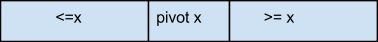
\includegraphics[scale = 0.7]{sort_quick_partition}\\
  \caption{Quick sort partition}\label{fig.sort.quick.partition}
\end{figure}
2 Conquer: recursively sort 2 subarrays\\
3 Combine: trivial(nothing to do for the combine)

\textbf{key step in quicksort is partition step}\\
快排在递归中也会进行partition\\
key: linear-time $\Theta(n)$ partitioning subroutine
\begin{verbatim}
Partition(A,p,q) //A[p...q]
x← A[p]  //pivot A[p]
i ← p
for j← p+1 to q{
    if A[j]<=x{
		i← i+1 //i加上1之后就到了大于x的那部分, 然后再将A[j] 交换到i 位置,loop invariant 保持
		exchange A[i] with A[j]
    }//end if
}//end for
exchange A[p] with A[i] // 将pivot 交换到中间, 完成partition 的任务
return i  //end function
\end{verbatim}

\begin{figure}[htbp]
  \centering
  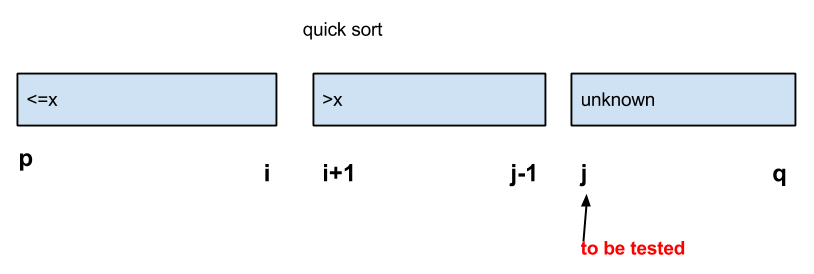
\includegraphics[scale = 0.7]{sort_quick_loopInvariant}\\
  \caption{Quick sort loop invariant}\label{fig.sort.quick.loopInvariant}
\end{figure}
At the beginning of each iteration of the loop, loop invariant
\begin{itemize}
\item if $k \in [p,i]$,then $A[k] \leq x$ and $A[p]=x$
\item if $k \in [i+1,j-1]$,then $A[k] >x$
\item if $k \in [j,q]$,then $A[k]$ unknown
\end{itemize}

running time  $T(n)\Theta(n)$  (只需要遍历一遍)
Ex: $2 8 7 1 3 5 6 4$\\
在这个例子中, 最后一个元素被选为pivot, 实际上pivot位于$p$或者$r$处都可以
\begin{figure}[htbp]
  \centering
  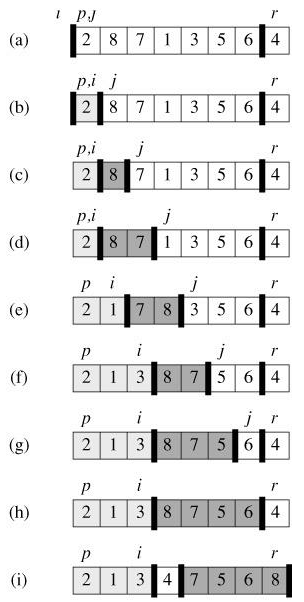
\includegraphics[scale = 0.7]{sort_quick_example}\\
  \caption{Quick sort example}\label{fig.sort.quick.example}
\end{figure}

\begin{verbatim}
Quicksort(A,p,q)
if p<q{
	r←Partition(A,p,q)
	Quicksort(A,p,r-1)
	Quicksort(A,r+1,q)
}
Initial call: Quicksort(A,1,n)
\end{verbatim}

\subsection{Analysis}
当元素数目较少时,可以换用其他更快更直接的算法,这样可以避免再简单的情况下也进行递归\\
同时,这是一个tail recursion(尾递归),所以可以使用certain tail recursion optimizations

\textbf{worst-case time}\\
-input sorted or reverse sorted 元素都被分到了一边\\
so one side of partition has no elems, the other side has $n-1$ elems\\
每次递归只减少了$1$,所以递归次数非常多\\
$T(n)
= \Theta(n)+T(0)+T(n-1)
= \Theta(n) + \Theta(1)+T(n-1)
=T(n-1) + \Theta(n)$\\
式中$\Theta(n)$表示partition所需要的时间\\
使用递归树得到时间复杂度为:$T(n)=\Theta(n^2)$

\textbf{best-case analysis(intuition only!)}\\
if we are really lucky, partition splits array $n/2:n/2$\\
$T(n)=\Theta(n)+2T(n/2)=\Theta(n\lg n)$  和merge sort一样

\textbf{Partition $1/10:9/10$}\\
$T(n)=T(n/10)+T(9n/10)+\Theta(n)$\\
用递归树得到\\
$T(n)<=(\log_{10/9}n*cn)+\Theta(n)=O(n\lg n)$\\
$T(n)<=(\log_{10}n*cn)+\Theta(n)=\Omega(n\lg n)$\\
$T(n)=\Theta(n\lg n)$\\
The reason is that any split of constant proportionality yields a recursion tree of depth $\Omega(\lg n)$ whenever the split has constant proportionality.

Suppose we alternate \textit{lucky, unlucky, lucky}...\\
$L(n)=2U(n/2)+\Theta(n)$	lucky的后面是两个unlucky\\
$U(n)=L(n-1)+\Theta(n)$	unlucky\\
Then
$$
\begin{aligned}
L(n)
&=2U(n/2)+\Theta(n) \\
&=2(L(n/2 - 1) +\Theta(n/2))+\Theta(n)\\
&=2L(n/2 - 1) + \Theta(n)\\
&=\Theta(n\lg n)  \eqnote{lucky}
\end{aligned}
$$

Suppose we alternate \textit{unlucky, lucky, unlucky, lucky}...
$$
\begin{aligned}
U(n)
&=L(n-1) + \Theta(n) \\
&=[2U((n-1)/2) + \Theta(n)] +\Theta(n)\\
&=2U((n-1)/2)) + \Theta(n)\\
&=2U(n/2) + \Theta(n)\\
&=\Theta(n\lg n)  \eqnote{lucky}
\end{aligned}
$$

So when we alternate lucky, unlucky, lucky...,we are lucky\\
Or we alternate unlucky, lucky, unlucky, lucky..., we are luck too.\\
So how do we ensure that we are usually lucky? \\
Because if the input is already sorted or reverse sorted, we are going to be unlucky.\\
1.randomly arrange the elements\\
2.randomly choose the pivot

\subsection{Random quicksort}
pick the pivot randomly\\
选择好之后,把这个选中的与array的第一个元素交换位置,这样这个随机选择的pivot就到了array的第一位置,然后再运行Partition函数
\begin{itemize}
\item 运行时间不取决于输入数据的顺序
\item 对输入序列的分布不用做出假设
\item 不存在特定的输入序列会引起worst-case
\item worst-case determined only by random number generator
\end{itemize}

\subsection{Median-of-3 Pivot}
For example, the median-of-3 pivot approach selects three candidate pivots and uses the median one.
If the three pivots are chosen from the first, middle and last positions, then it is easy to see that for the already sorted array,
this will produce an optimum result: each partition will be exactly half ($\pm$ one element) of the problem and we will need exactly ceiling($\log n$) recursive calls.

\subsection{Random method analysis}
Random variable(随机变量) for running time assuming that random numbers are independent.\\
I want to know where I pivoted. 设这个pivot 的位置为随机变量$k$\\
So for $k=0, 1...n-1$ let\\
$x_k=1$ if partition generates a $k: n-k-1$ split, (pivot 算一个数, 所以两者加起来是n-1)\\
$x_k=0$ otherwise\\
这样一个partition,就产生了$n$个random variable,其中只有一个是$1$,其余的都是$0$.\\
例如如果产生的partition为$5:n-6$,那么只有$x_5=1,x_i=0 (i \in  [[0,n-1]]$ and $i!=5)$\\
this type of random variable is called \textbf{indicator random variable}

the expected value of $x_k:\\
E[x_k]=0*P(x_k =0)+1*P(x_k =1) = P(x_k =1) =1/n$\\
因为每一个数$k$ 都有可能取到, 而且概率是一样的, 所以每个数的概率都是 $1/n$
$$
T(n) =
\left\{
  \begin{array}{ll}
		  T(0) + T(n-1) \si 0:n-1 split \\
		  T(1) + T(n-2) \si 1:n-2 split \\
            \vdots \\
		  T(n-1) + T(0) \si n-1:0 split
  \end{array}
\right.
$$
所以这就是T(n)的递归,但是这个递归很麻烦,这里我们就可以看到indicator random variable的优美性,我们将使用indicator random variable将这个递归reduce to(规约到数学上)
$$
T(n) = \sum_{k=0}^{n-1} x_k (T(k) + T(n-k-1) + \Theta(n))
$$

$T(n)$的期望
\begin{equation}
\begin{split}
   E[T(n)] & =E[\sum_{k=0}^{n-1}x_k(T(k)+T(n-k-1)+\Theta(n))] \\
           & =\sum_{k=0}^{n-1}E[x_k(T(k)+T(n-k-1)+\Theta(n))]\\
           & \text{$x_k$随机变量独立于任何其他的partitions, 也就是说$x_k$ 区别于}\\
           & \text{其他递归调用,所以积的期望等于期望的积}\\
           & =\sum_{k=0}^{n-1}E[x_k]*E[(T(k)+T(n-k-1)+\Theta(n))]\\
           & = \frac{1}{n}\sum_{k=0}^{n-1}E[(T(k)] + \frac{1}{n}\sum_{k=0}^{n-1}E[T(n-k-1)] +\frac{1}{n}\sum_{k=0}^{n-1}\Theta(n)\\
           & =\frac{2}{n}\sum_{k=0}^{n-1}E[(T(k)] +\Theta(n)
\end{split}
\end{equation}

$x_k$ 是对$n$进行partition时产生的一个indicator random variable也就是说$x_k$是和$T(n)$ 是相关的, 而后面的$T(k)$ 与$T(n-k-1)$是在有了$x_k$ 之后, 也就是产生了一个$k,n-k-1$的分割后, 对产生的两个新的分割求时间时, 又会产生新的indicator: $x'_k$\\
所以$x_k$ 与$T(k), T(n-k-1)$是相互独立的, 可以运用概率的乘法原则

Absorb $k=0,1$ terms into $\Theta(n)$ for tech convenence,(两个常量加进去不影响$\Theta(n)$)
$$
E[T(n)]=\frac{2}{n}\sum_{k=2}^{n-1}E[T(k)]+\Theta(n)
$$

Use fact\todo{how to prove?}
$$
\sum_{k=2}^{n-1}k\lg k \leq \frac{1}{2}n^2\lg n-\frac{1}{8}n^2
$$
To prove $E[T(n)]<=a*n\lg n$ for constant $a>0$ with the substitution method\\
$E[T(n)] \leq an \lg n –bn (a, b >0)$\\
.....\\
所以我们得到$T(n)$的期望值是$\Theta(n\lg n)$\\
so the running time of randomized quicksort is $\Theta(n\lg n)$

The version of PARTITION given in this chapter is not the original partitioning algorithm. Here is the original partition algorithm, which is due to T.Hoare:
\begin{verbatim}
HOARE-PARTITION(A, p, r)
 1  x ← A[p]
 2  i ← p - 1
 3  j ← r + 1
 4  while TRUE
 5      do repeat j ← j - 1
 6           until A[j] <= x
 7         repeat i ← i + 1
 8           until A[i] >= x
 9         if i < j
10            then exchange A[i] with A[j]
11            else return j
\end{verbatim}
Every element of $A[p ‥ j]$ is less than or equal to every element of $A[j +1 ‥ r]$ when HOARE-PARTITION terminates.\\
The HOARE-PARTITION procedure always places the pivot value (originally in $A[p]$) into one of the two partitions $A[p ‥ j]$ and $A[j + 1 ‥ r]$.

\subsection{Exercise}
[Exercises 7.4-5]
The running time of quicksort can be improved in practice by taking advantage of the fast running time of insertion sort when its input is "nearly" sorted.
When quicksort is called on a subarray with fewer than $k$ elements, let it simply return without sorting the subarray.
After the top-level call to quicksort returns, run insertion sort on the entire array to finish the sorting process.
Argue that this sorting algorithm runs in $O(nk + n \lg(n/k))$ expected time. How should k be picked, both in theory and in practice?

[Problems 7-6: Fuzzy sorting of intervals]
Consider a sorting problem in which the numbers are not known exactly. Instead, for each number, we know an interval on the real line to which it belongs.
That is, we are given n closed intervals of the form $[a_i, b_i]$, where $a_i \leq b_i$.
The goal is to fuzzy-sort these intervals, i.e.,to produce a permutation $〈i_1, i_2,\ldots, i_n〉$ of the intervals such that for $j = 1,2,\ldots,n$
there exist $c_j \in [a_{i_j}, b_{i_j}]$, satisfying $c_1 \leq c_2 \leq \cdots \leq c_n$.\\
1.	Design an algorithm for fuzzy-sorting $n$ intervals. Your algorithm should have the general structure of an algorithm that
quicksorts the left endpoints (the $a_i$ values), but it should take advantage of overlapping intervals to improve the running time.
(As the intervals overlap more and more, the problem of fuzzy-sorting the intervals gets easier and easier.
Your algorithm should take advantage of such overlapping, to the extent that it exists.)\\
2.	Argue that your algorithm runs in expected time $\Theta(n \lg n)$ in general, but runs in expected time $\Theta(n)$
when all of the intervals overlap (i.e., when there exists a value $x$ such that $x \in [a_i, b_i]$ for all $i$).
Your algorithm should not be checking for this case explicitly; rather, its performance should naturally improve as the amount of overlap increases.

\section{Heapsort}
Implementation of heap: tree or array\\
Max-heap: parent $\geq$ children,
	heapsort\\
Min-heap: parent $\leq$ children,
	priority queue

下面我们以Max-heap 进行讲解\\
Array n elements, leaves: $floor(n/2) + 1, floor(n/2) + 2, floor(n/2) + 3, \cdots, n$

The (binary) heap data structure is an array object that we can view as a nearly complete binary tree
\begin{verbatim}
PARENT(i)
   return floor(i/2)
LEFT(i)
   return 2i
RIGHT(i)
   return 2i + 1
\end{verbatim}

\begin{figure}[htbp]
  \centering
  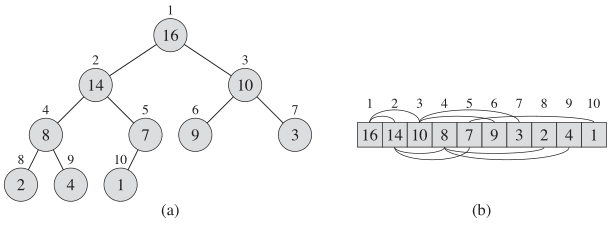
\includegraphics[scale = 0.7]{sort_heap_example}
  \caption{An example of heap}\label{fig.sort.heap.example}
\end{figure}

The height of a node: the length of the longest downward path to a leaf from that node\\
The depth of a node: the length of the path to its root\\
Root node has depth 0, leaf node has height 0

\subsection{Maintaining the heap property}
Its inputs are an array A and an index i into the array\\
A[i] "float down"

\begin{verbatim}
Max-heapify(A, i)
   l = left(i)
   r = right(i)
   if l <= A.heap-size and A[l] > A[i]
      largest = l
   else largest = i
   if r <= A.heap-size and A[r] > A[i]
      largest = r
   if largest != i
      exchange A[i] with A[largest]
      Max-heapify(A, largest)
\end{verbatim}

max heapify: correct a single violation of the heap property in a sub tree's root\\
\textbf{运行Max-heapify(A, i) 的前提条件precondition}: assume that the trees rooted at left(i) and right(i) are max-heaps

\begin{figure}[htbp]
  \centering
  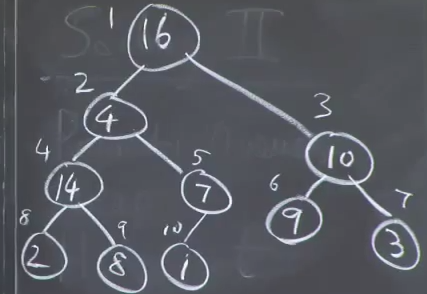
\includegraphics[scale = 0.7]{sort_heap_violation}
  \caption{An example of violation of heap property}\label{fig.sort.heap.violation}
\end{figure}
图\ref{fig.sort.heap.violation}中的第二个节点violates the max heap property, 所以我们可以调用max-heapify(A, 2), 修复好这个之后, 再进行检查直到不出现violation 为止

The children's subtrees each have size at most $2n/3$\todo{not understood}—the worst case occurs when the bottom level of the tree is exactly half full—and therefore we can describe the running time of MAX-HEAPIFY by the recurrence\\
$T(n) \leq T(2n/3) +\Theta(1)$\\
master theorem => $T(n) = O(\lg n)$

add a new item : place the new item at the last position(向左向下走知道不能继续前进), 然后进行修复, compare it with its parent, if it is larger than its parent, exchange them 向上继续进行这个比较直到不违反heap的性质, 也就是向上修复\\
delete the root : 将最后一个节点的值赋给root, 然后向下进行修复

\subsection{Building a heap}
build-max heap: produce a max heap from an unordered array

The elements in the subarray $A[(floor(n/2)+ 1)…n]$ are all leaves of the tree\todo{how to prove}\\
而leaf 已经是max-heap了, 因为leaf 没有children

The procedure BUILD-MAX-HEAP goes through the remaining nodes of the tree and runs MAX-HEAPIFY on each one
\begin{verbatim}
Build-Max-heap(A)
A.heap-size = A.length
    for i = floor(A.length / 2) downto 1
        Max-heapify(A, i) //每次调用max-heapify 之前, 都是满足max-heapify的precondition的
\end{verbatim}

Each call to MAX-HEAPIFY costs $O(\lg n)$ time, and BUILD-MAX-HEAP makes $O(n)$ such calls. Thus, the running time is $O(n\lg n )$. This upper bound, though correct, is not asymptotically tight.

但是我们可以发现:\\
max-heapify takes $O(1)$ for nodes that are one level above the leaves\\
and in general $O(l)$ time for nodes that re l levels above the leaves

an n-element heap has height $floor(\lg n )$ and at most $ceil(n/(2^{h+1}))$ nodes of any height $h$\todo{need proof}

$$
\sum_{h=0}^{\lfloor \lg n \rfloor} \lceil \frac{n}{2^{h+1}} \rceil O(h)
=
O(n \sum_{h=0}^{\lfloor \lg n \rfloor} \frac{h}{2^h})
$$

$$
\sum_{h=0}^{\infty} \frac{ h}{2^h} = \frac{1/2}{(1 - 1/2)^2} = 2
$$
Thus, we can bound the running time of BUILD-MAX-HEAP as
$$
O(n \sum_{h=0}^{\lfloor \lg n \rfloor} \frac{h}{2^h})
= O(n \sum_{h=0}^{\infty} \frac{h}{2^h})
= O(n)
$$

Hence, we can build a max-heap from an unordered array in linear time

\subsection{The heapsort algorithm}
build-max-heap from unordered array\\
find max element $A[1]$\\
swap elements $A[n]$ with $A[1]$, now max element is at the end of the array\\
Discard node $n$ from heap,\\
New root may violate max heap property, fix it

\begin{verbatim}
Heapsort(A)
    Build-Max-heap(A)
    for i = A.length downto 2
        exchange A[1] with A[i]
        A.heap-size = A.heap-size - 1
        Max-heapify(A, 1)
\end{verbatim}

把$A[1]$ 也就是最大值挪到最后一个位置, 同时将heap 的大小减一, 这样最大值就从heap 从取出来了并被放在了正确的位置上, 然后再修复这个heap; 然后再最大值重复这个操作

time $O(n\lg n )$\\
in place sort

\subsection{Priority queues}
max-priority queue, min-priority queue\\
we can use a heap to implement a priority queue

\begin{verbatim}
HEAP-MAXIMUM(A)
    return A[1]
\end{verbatim}
heap-maximum: $\Theta(1)$ time

\begin{verbatim}
HEAP-extract-MAX(A)
    if A.heap-size < 1
        error "heap underflow"
    max = A[1]
    A[1] = A[A.heap-size]
    A.heap-size = A.heap-size - 1
    MAX-HEAPIFY(A,1)
    return max
\end{verbatim}
heap-extract-max: $O(\lg n )$ time

\begin{verbatim}
HEAP-INCREASE-KEY(A,i,key)
    if key < A[i]
        error "new key is smaller than current key"
    A[i] = key
    while i > 1 and A[PARENT(i)] < A[i]
        exchange A[i] with A[PARENT(i)]
        i = PARENT(i)
\end{verbatim}
HEAP-INCREASE-KEY: $O(\lg n )$ time

\begin{verbatim}
MAX-HEAP-INSERT(A,key)
    A.heap-size = A.heap-size + 1
    A[A.heap-size] = -\infty
    HEAP-INCREASE-KEY(A,A.heap-size,key)
\end{verbatim}
MAX-HEAP-INSERT: $O(\lg n )$ time

\section{线性时间排序}
\begin{itemize}
\item quicksort $\Theta(n\lg n )$  randomized
\item heapsort $\Theta(n\lg n )$ 堆排序
\item merge sort $\Theta(n\lg n )$
\item insertion sort $\Theta(n^2)$
\end{itemize}

can we do better than $\Theta(n\lg n )$?\\
comparison sorting model\\
only use comparisons to determine relative order of elements

\subsection{decision tree model 决策树}
Ex: sort $<a_1, a_2, a_3>$

In general $<a_1,a_2...,a_n>$
\begin{itemize}
\item each internal node labeled $i, j$ means compare $a_i$ vs. $a_j$
\item left subtree $a_i <= a_j$
\item right subtree $a_i > a_j$
\item each leaf gives a permutation of the array
\end{itemize}

图\ref{fig.decision_tree.example}是一个决策树的例子
\begin{figure}[htbp]
  \centering
  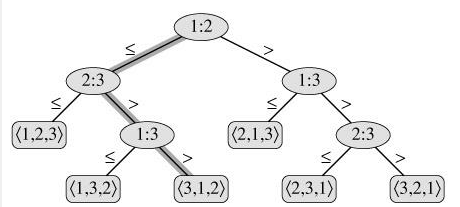
\includegraphics[scale = 0.7]{decision_tree_example}\\
  \caption{Decision tree example}\label{fig.decision_tree.example}
\end{figure}

\textbf{A lower bound for the worst case}\\
The length of the longest path from the root of a decision tree to any of its reachable leaves represents the worst-case number of comparisons. Consequently,
the worst-case number of comparisons for a given comparison sort algorithm equals the height of its decision tree. A lower bound on the heights of all decision trees in which each permutation appears as a reachable leaf is therefore a lower bound on the running time of any comparison sort algorithm. The following theorem establishes such a lower bound.

[Theorem 8.1] Any comparison sort algorithm requires $\Omega(n \lg n)$ comparisons in the worst case.\\
Proof: From the preceding discussion, it suffices to determine the height of a decision tree in which each permutation appears as a reachable leaf.\\
Consider a decision tree of height h with l reachable leaves corresponding to a comparison sort on n elements.
Because each of the $n!$ permutations of the input appears as some leaf, we have $n! \leq l$.(至少含有$n!$ 个leaves)
Since a binary tree of height h has no more than $2^h$ leaves, we have\\
$n! \leq l \leq 2^h$,
which, by taking logarithms, implies\\
$h \geq \lg (n!) = \Omega(n\lg n)$ (Stirling's approximation $n! \simeq (n/e)^n$

\subsection{Counting sort计数排序}
Element $\in [0, k]$ for some integer $k$. \\
When $k = O(n)$, the sort runs in $\Theta(n)$ time.\\
The \textbf{basic idea} of counting sort is to \textbf{determine, for each input element $x$, the number of elements less than $x$}.
This information can be used to place element $x$ directly into its position in the output array.\\
For example, if there are $17$ elements less than $x$, then $x$ belongs in output position $18$.
This scheme must be modified slightly to handle the situation in which several elements have the same value,
since we don't want to put them all in the same position.

input array $A[1,\ldots, n]$, and thus $length[A] = n$.\\
the array $B[1,\ldots,n]$ holds the sorted output, \\
the array $C[0,\ldots,k]$ provides temporary working storage.

\begin{verbatim}
COUNTING-SORT(A, B, k)
 1  for i ← 0 to k
 2     do C[i] ← 0
 3  for j ← 1 to length[A]
 4     do C[A[j]] ← C[A[j]] + 1
 5  // C[i] now contains the number of elements equal to i.
 6  for i ← 1 to k
 7     do C[i] ← C[i] + C[i - 1]
 8  // C[i] now contains the number of elements leqi
 9  for j ← length[A] downto 1
10     do B[C[A[j]]] ← A[j]
11        C[A[j]] ← C[A[j]] - 1
\end{verbatim}

An important property of counting sort is that it is \textbf{stable}.

Analysis\\
line $1-2 \Theta(k)$\\
line $3-4 \Theta(n)$\\
line $6-7 \Theta(k)$\\
line $9-11 \Theta(n)$\\
Overall time$\Theta(n+k)$\\
在实际上, 当 $k\Theta(n)$ 时, 我们才采用 counting sort

[Exercises 8.2-3] Suppose that the for loop header in line $9$ of the COUNTING-SORT procedure is rewritten as
\begin{verbatim}
9	 for j ← 1 to length[A]
\end{verbatim}
Show that the algorithm still works properly. Is the modified algorithm stable?\\
凭直觉来看, 不是stable

\subsection{Radix sort基数排序}
LSD(Least Significant Digit first)的基数排序适用于位数小的数列,如果位数多的话,使用MSD的效率会比较好.\\
MSD(Most Significant Digit first)的方式与LSD相反,是由高位数为基底开始进行分配,但在分配之后并不马上合并回一个数组中,
而是\textbf{在每个"桶子"中建立"子桶"},将每个桶子中的数值按照下一数位的值分配到"子桶"中.在进行完最低位数的分配后再合并回单一的数组中.

这里讲到的是LSD

\subsubsection{说明}
其原理在于对于待排序的数据,\textbf{整体权重未知}的情况下,
先按权重小的因子排序,然后按权重大的因子排序.\\
例如比较时间,先按日排序,再按月排序,最后按年排序,仅需排序三次.

但是如果先排序高位就没这么简单了.\\
\textbf{基数排序源于老式穿孔机,排序器每次只能看到一个列(这就是一个整体权重未知的例子)},
很多教科书上的基数排序都是对数值排序(这样意义不大),数值的大小是已知的,与老式穿孔机不同.将数值按位拆分再排序,是无聊并自找麻烦的事.算法的目的是找到最佳解决问题的方案,而不是把简单的事搞的更复杂.

\textbf{基数排序更适合用于对时间,字符串等这些整体权值未知的数据进行排序.}
这时候基数排序的思想才能体现出来,例如字符串,如果从高位(第一位)往后排就很麻烦.
而反过来,先对影响力较小,的低位(最后一位)进行排序就非常简单了.
这时候基数排序的思想就能体现出来.

$d$ 位数字, 每一位数字可以取 $k$ 个不同的数, 例如$0$ 到$9$ 十个数, 那么$k=10$
\begin{verbatim}
RADIX-SORT(A, d)
    for i from 1 to d:
        do use a stable sort to sort array A on digit i
\end{verbatim}

\subsubsection{Analysis}
time:$\Theta(d(n+k))$

证明:correctness\\
induct on digit position $t$\\
assume by induction 前$t-1$位已经排好序, 我们需要对第$t$位进行排序\\
1, if two elements have same $t$th digit, stability $\Rightarrow$ same order $\Rightarrow$ sorted order\\
2, if different $t$th digit $\Rightarrow$ sorted order

---use counting sort digits\\
---suppose we have $n$ integers each $b$ bits ( $range=[0,2^b-1]$, non-negative)\\
---split into $b/r$ "digits" each $r$ bits (将$r$个bits组合成一个大的"bit")\\
time $O(b/r*(n+k))=O(b/r*(n+2^r))$\\
对r求导, 令其为零求得此时的r值 $r=\lg n$\\
得到$O(bn/\lg n )$

if number in range $0,2^b-1$ then $time = O(dn)$\\
if  $d=O(1)$ then $time=O(n)$

而且只要$d$小于$\lg n$, 就可以击败comparison sort\\
但是在实际上, counting sort is not very good on a cache, in practice, radix sort is not that fast, unless your numbers are really small.\\
但是在理论上, 这个算法很优美

Finally, if you have arbitrary integers, that are one word length long, and you can manipulate a word in constant time.\\
Then the best algorithm we known for sorting runs $n*\sqrt{\lg\lg n }$, and this is a randomized algorithm and very complicated\\
有另外一个算法$n*lg(\lg n )$ worst case, 这篇论文应该可以看懂

\section{Order statistics}
given n elements\\
find $k$th smallest element\\
naive algorithm: sort and return $A[k]$\\
$k=1$ minimum\\
$k=n$ maximum\\
median 中位数 $k=floor((n+1)/2)$ or $ceil((n+1)/2)$

randomized divide and conquer\\
random-select \\
$\Theta(n)$ expected running time\\
$\Theta(n^2)$ worst-case  差不多是$1/n^n$ 的概率\\
intuition for analysis\\
(we assume 所有数都不等)\\
lucky case: $1/10, 9/10$\\
$T(n) \leq T(9/10n)\Theta(n)$  假设第$i$小的位于$9/10$部分\\
unlucky case: $0, n-1$\\
$T(n)=T(n-1)\Theta(n)\Theta(n^2)$

indicator random variable\\
let $T(n)$  be the random variable for running time of random-select\\
define indicator random variable $x_k, k \in [0, n-1]$\\
$x_k = 1$	if partition generates an $k$ to $n-k-1$ splits \\
$x_k = 0$	otherwise

substitution method , $E[T(n)] \leq cn$\\
$3/8n^2$ induction to get $3/8$

worst-case linear time order statistics

Why do we group in $5$ numbers, not $3$ or $7$ or others?\\
$3$是不行的, $7$也行, 但是对于效率没有什么提升

\section{Appendix}
\subsection{Summations}
\subsubsection{Approximation by integrals}
$$
\sum_{k=1}^n \frac{ 1}{k} \geq \int_1^{n+1}\frac{1}{x}dx = \ln(n+1)
$$

$$
\sum_{k=2}^n \frac{ 1}{k} \leq \int_1^{n}\frac{1}{x}dx = \ln n
$$
which yields the bound
$$
\sum_{k=1}^n \frac{ 1}{k} \leq \ln n + 1
$$

\subsection{Relations}
$v_0',v'_0$
A binary relation $R$ on two sets $A$ and $B$ is a subset of the Cartesian product$A \times B$
If $(a, b) \in R$, we sometimes write $a R b$. When we say that R is a binary relation on a set $A$, we mean that R is a subset of $A \times A$. For example, the "less than" relation on the natural numbers is the set $\{(a, b) : a, b$ in $N$ and $a < b\}$. An n-ary relation on sets $A_1, A_2,\ldots, A_n$ is a subset of $A_1 \times A_2 \times \cdots \times  A_n$.

A binary relation $R \subseteq A \times A$ is reflexive if
$a R b$ implies $b R a$ for all $a,b \in A$
\subsection{Probability}
$$
Pr(A\cap B)=\frac{Pr(A)*Pr(B \cap A)}{Pr(B)}
$$

$$
B=(B \cap A)\cup (B \cap \bar{A})
$$

$$
Pr(B)=Pr(B \cap A)+Pr(B \cap \bar{A})
=Pr(A)*Pr(B|A)+Pr(\bar{A})*Pr(B|\bar{A})
$$

$$
Pr(A\cap B)=\frac{Pr(A)*Pr(B \cap A)}{Pr(A)*Pr(B|A)+Pr(\bar{A})*Pr(B|\bar{A})}
$$

\end{document}
